\chapter{Dicas de Latex e Normas ABNT}
Esta capítulo apresenta as coisas básicas que precisamos saber para fazer um TCC com Latex utilizando este modelo.

\section{O Básico do Latex}
Novo parágrafo pode ser feito por meio do comando par. \par
Outra forma é deixando uma linha em branco entre dois parágrafos.

Tudo o que está a direita de um \% é um comentário.
% Isto é um comentário
Para inserirmos o símbolo de porcento de forma proposital, precisamos colocar a barra invertida antes: 90\%.

Os caracteres \& \$ \# \% \_ \{ \} \^{} \~{} $\backslash$ são todos especiais e precisam ser escritos como comandos (com uma barra antes).
% tem um web app para ajudar a encontrar outros símbolos neste endereço: http://detexify.kirelabs.org/classify.html

Aspas são digitadas com duas crases no início e duas aspas simples no final: ``Texto entre aspas''; ou com o comando say: \say{Texto entre aspas}.

Estilos de fontes: \emph{ênfase} (sempre destaca o texto, mesmo que este já esteja em negrito/itálico), \textbf{negrito}, \textit{itálico}, \textrm{romano}, \textsf{sans serif}, \texttt{máquina de escrever}, \textsc{caixa alta}.

Capítulos, seções e subseções são inseridas com:
\begin{verbatim}
\chapter{Um Capítulo} -> 1 Um Capítulo
\section{Uma Seção} -> 1.1 Uma Seção
\subsection{Uma Subseção} -> 1.1.1 Uma Subseção
\subsubsection{Uma Subsubseção} -> 1.1.1.1 Uma Subsubseção
\chapter*{Um Capítulo} -> Um Capítulo sem numeração
\end{verbatim}
Não se deve utilizar mais do que 4 níveis.

Ambientes são utilizados para definir uma região do texto que haverá tratamento especial:

\begin{verbatim}
O ambiente verbatim significa "ao pé da letra". 
Ex.: & $ # % _ { } ^ ~ $
\end{verbatim}

\begin{center}
O ambiente center escreve centralizado.
\end{center}

\begin{quote}
O ambiente quote é útil para fazer citações.
\end{quote}

Esta é a forma como se descreve itens:
\begin{description}
\item[Item 1] Isto significa uma coisa.
\item[Item 2] Este significa outra coisa.
\end{description}

Esta é a forma como se cita itens:
\begin{itemize}
\item Item 1;
\item Item 2.
\end{itemize}

E esta é a forma como se enumera itens:
\begin{enumerate}
	\item Qual a alternativa correta?
		\begin{enumerate}
			\item esta.
			\item ou esta.
		\end{enumerate}
\end{enumerate}

Fórmulas matemáticas são colocadas dentro de um ambiente matemático. Tudo neste ambiente é considerado elemento numérico e possui uma formatação diferente. Os comandos aceitos também podem mudar.

Equações matemáticas em destaque são inseridas da seguinte maneira:

% tem um web app para ajudar a fazer equações neste endereço: http://mathurl.com/
% ou aqui: http://webdemo.visionobjects.com/#/demo/equation
$$
x=\frac{-b\pm\sqrt{b^2-4ac}}{2a}.
$$

ou 

\begin{equation}
\begin{array}{rcl}
x_2 - x_1 &\geq& b_1 r_1\\
x_2 - x_1 &\geq& b_2 r_2\\
x_2 - x_1 &\geq& b_n r_m\\
b_1 + b_2 + ... + b_n &=& 1
\end{array}
\end{equation}

enquanto equações inline são feitas desta forma: $r_i (1\leq i \leq m)$.

\section{Convenções}
Escreva o título e os capítulos, seções, subseções, etc. sempre com a primeira letra de cada palavra importante em Maiúsculo e o restante em minúsculo. O Latex se encarregará de deixar tudo MAIÚSCULO onde for necessário.

Nenhuma seção deve ficar sem texto.

Utilize siglas para não ter de repetir muitas vezes o mesmo texto. Neste caso, na primeira ocorrência coloque o significado antes e a sigla entre parênteses (aproveitando também para adiciona-la à lista de siglas). Nas demais ocorrências, apenas coloque a sigla. 
Ex.: ...com a execução do algoritmo de \textit{Threshold Accepting} (TA) sobre um circuito. A versão do algoritmo de TA utilizada...

Palavras em \textit{English} ou outra língua estrangeira devem estar em itálico. Utilize \textbf{negrito} quando for necessário destacar alguma coisa.

\section{Figuras e Tabelas}

Todas as figuras e tabelas devem estar referenciadas no texto e com a descrição acima delas. Não são permitidos outros nomes tais como: quadro, imagem, etc. Comece a descrição com letra maiúscula e faça o restante em minúscula (exceto siglas), terminando com um ponto final.

Se buscada em alguma obra publicada, a citação deve sempre aparecer. Pode ser colocada entre parênteses, como no exemplo da Figura \ref{fig:dsp2}, ou preferencialmente abaixo após a palavra "Fonte: ", como no exemplo da Tabela \ref{tab:comp1} e da Figura \ref{fig:dsp}. Observando que na LISTA DE FIGURAS/TABELAS a fonte/citação não deve aparecer.

É possível colocar as figuras de lado e também redimensiona-las através dos parâmetros do Latex, como nos exemplos das Figuras \ref{fig:dsp} e \ref{fig:dsp2}. Dê preferência por imagens vetoriais ou em PDF, para não perder qualidade. Procure deixar os textos das figuras com o mesmo tamanho das letras no restante do documento.

\begin{figure} % [h] -> utilize este parâmetro para forçar nesta posição
    \center{
    \caption{Segundo a ABNT, a descrição deve ficar acima da figura.}
    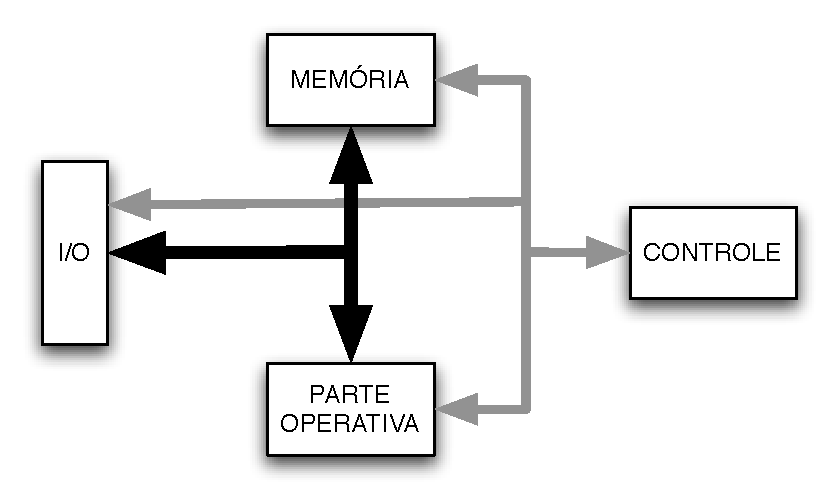
\includegraphics[width=20em]{figuras/dsp}\\
    Fonte: Elaborado pelo autor.}
    \label{fig:dsp}
\end{figure}

\begin{sidewaysfigure}
    % entre colchetes a descrição que vai para a lista de figuras, sem citação (parâmetro opcional mas que é necessário devido a norma da ABNT)
    \caption[Descrição com citação]{Descrição com citação \cite{artigo}.}
    \centerline{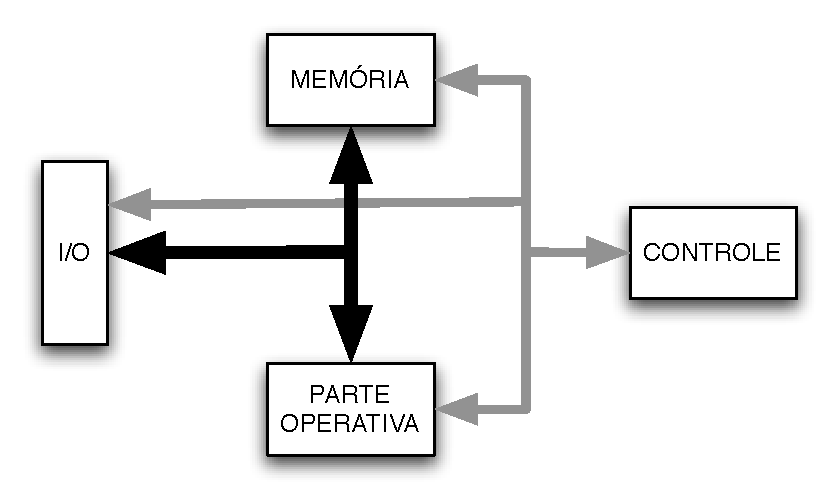
\includegraphics[width=40em]{figuras/dsp}}
    \label{fig:dsp2}
\end{sidewaysfigure}

As tabelas devem ser ``abertas'' dos lados (sem as linhas laterais), como no exemplo da Tabela \ref{tab:comp1}, isto torna a imagem mais limpa e clara.

% tem um web app para ajudar a fazer tabelas no Latex neste endereço: http://truben.no/latex/table/
\begin{table}
    \centering
    \scalefont{0.93} %necessário eventualmente para reduzir o tamanho da tabela
    \caption{Comparação entre X e Y.}
    \begin{tabular}{c|c|c|c|c|c} \hline
        \multirow{2}{*}{\textbf{Célula}} & \multirow{2}{*}{\# \bf{Trans.}} & \multicolumn{3}{|c|}{\bf{Largura} ($\mu m$)} & \bf{Tempo Exec. (s)}\\ \cline{3-6} 
         &  & Std. Cell & ASTRAN & \% & ASTRAN \\ \hline \hline
        AND2X4& 6 & 1 & 1,2 & 20 & 10 \\ \hline
        FAD1X4& 28 & 3,6 & 4 & 12 & 750\\ \hline
        FAD1X9& 28 & 4,2 & 4,2 & 0 & 1800\\ \hline
        HAD1X9& 14 & 2,4 & 2,4 & 0 & 30\\ \hline
        HAD1X18& 18 & 2,8 & 2,8 & 0 & 205\\ \hline
        INVX0 & 2 & 0,6 & 0,6 & 0 & 1\\ \hline
        TOTAL& - & 28 & 29 & 3,6 &-\\ \hline
    \end{tabular}
    {\\ Fonte: \cite{artigo}}
    \label{tab:comp1}
\end{table}

\section{Citações}
Há duas formas de se fazer uma citação: a citação indireta ou livre e a citação direta ou textual. Todas as citações devem trazer a identificação de sua autoria.

No Latex, inserimos citações utilizando o formato bibtex. Para tanto, precisamos cadastrar os dados da citação no arquivo .bib e em seguida citarmos no .tex com o comando cite. Colocar preferencialmente em ordem cronológica, com o mais recente por último \cite{livro, artigo, tese, capitulo, paper, site, apresentacao}.

\subsection{Citação Indireta}
Aquela citação na qual expressamos o pensamento de outra pessoa com nossas próprias palavras. Por esta razão seu uso é mais recomendado, pois demostra interpretação do autor sobre a obra citada. Ex.:

Segundo o trabalho de Silva e Santos \citeyearpar{artigo}, o céu é azul porque...

O céu é azul porque... \cite{artigo}.

\subsection{Citação Direta}
São aquelas em que se transcreve exatamente as palavras do autor citado. As citações diretas ou textuais podem ser breves ou longas. São consideradas breves aquelas cuja extensão não ultrapassa três linhas e devem vir entre aspas. As citações com mais de três linhas são chamadas de longas (sem aspas) e devem receber um destaque especial com recuo.  Ex.:

Segundo Silva, ``Quando a luz passa através de um prisma, seu espectro é dividido em sete cores monocromáticas'' \citeyearpar{artigo}.

\begin{quote}
Quando a luz passa através de um prisma, seu espectro é dividido em sete cores monocromáticas, eis que surge um arco-íris de cores. A atmosfera faz o mesmo papel do prisma, atuando onde os raios solares colidem com as moléculas de ar, água e poeira e são responsáveis pela dispersão do comprimento de onda azul da luz. \cite{artigo}
\end{quote}

Havendo supressão de trechos dentro do texto citado, faz-se a indicação com reticências entre colchetes [...]. De forma similar, para interpelação, acréscimo ou comentário durante a citação, deve-se fazê-lo também entre colchetes. No início ou no fim da citação, as reticências são usadas apenas quando o trecho citado não é uma sentença completa.Ex.:

``Também chamado de corpo do trabalho, [o desenvolvimento] tem por finalidade expor [...] a explicitação do assunto a ser abordado...'' \cite{artigo}.

\section{Notas de Rodapé}
As notas de rodapé\footnote{Nota sobre a palavra rodapé} são usadas nos documentos impressos para explicar ou fazer comentários detalhados.
